\section{결과}\label{sec:results}
\subsection{공칭 추종과 튜닝}
\Cref{tab:nominal} 및 \cref{fig:nominal,fig:tuning}에 기존 및 재튜닝 비교를 나타냈다. 기존 LQI의 공칭 IAE가 7304.8~$^\circ$C s로 가장 작지만, 동일 예산 튜닝 후 공칭 훈련 시나리오 순위는 LQR(7180.2), LQI(7236.8), PID(7455.0)이다. 이는 선언한 목적함수 아래의 조건부 순위이며 보편적 우수성의 증거가 아니다.
\begin{table}[!htbp]\centering\caption{Rust로 생성한 기존 및 재튜닝 공칭 비교.}\label{tab:nominal}\resizebox{\linewidth}{!}{\begin{tabular}{llrrr}\toprule
Design & Controller & IAE ($^\circ$C s) & RMSE ($^\circ$C) & Settling (s) \\
\midrule
Original & PID & 7584.2 & 6.227 & 600 \\
Original & LQR & 8068.3 & 6.272 & 837 \\
Original & LQI & 7304.8 & 6.208 & 517 \\
Retuned & PID & 7455.0 & 6.221 & 605 \\
Retuned & LQR & 7180.2 & 6.207 & 502 \\
Retuned & LQI & 7236.8 & 6.207 & 508 \\
\bottomrule\end{tabular}
}\end{table}
\begin{figure}[!htbp]\centering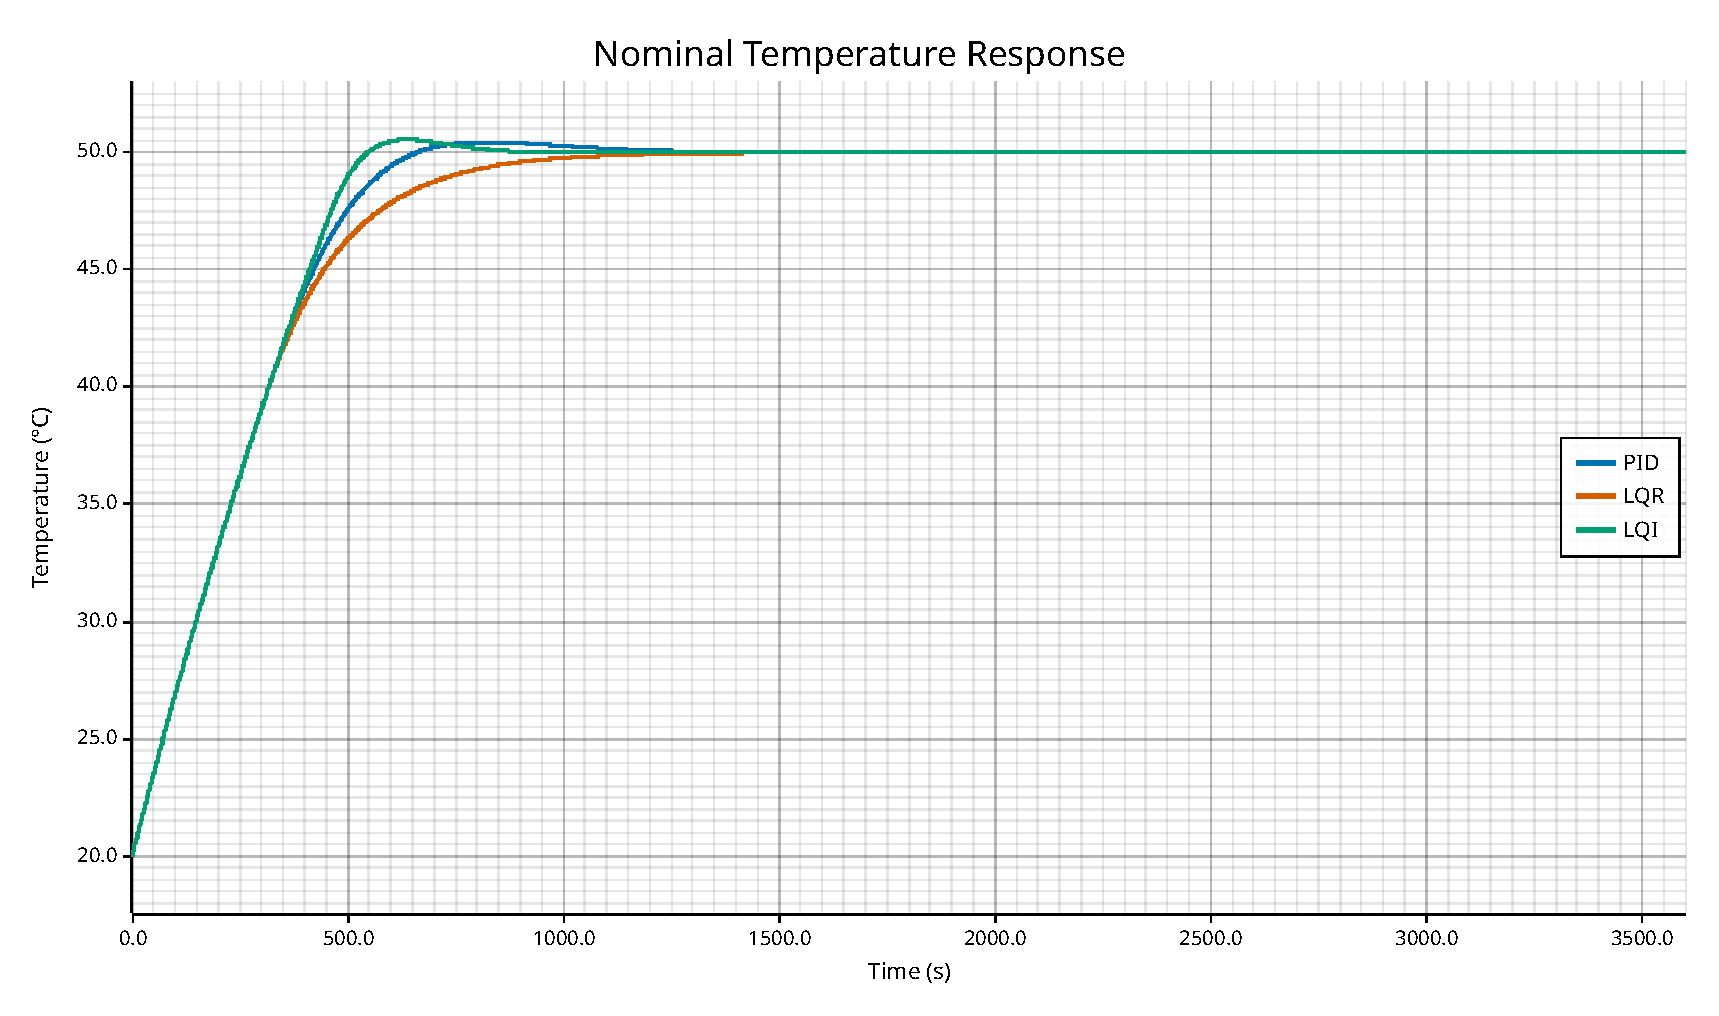
\includegraphics[width=\linewidth]{figures/nominal-temperature.pdf}\caption{기존 제어기의 공칭 추종.}\label{fig:nominal}\end{figure}
\begin{figure}[!htbp]\centering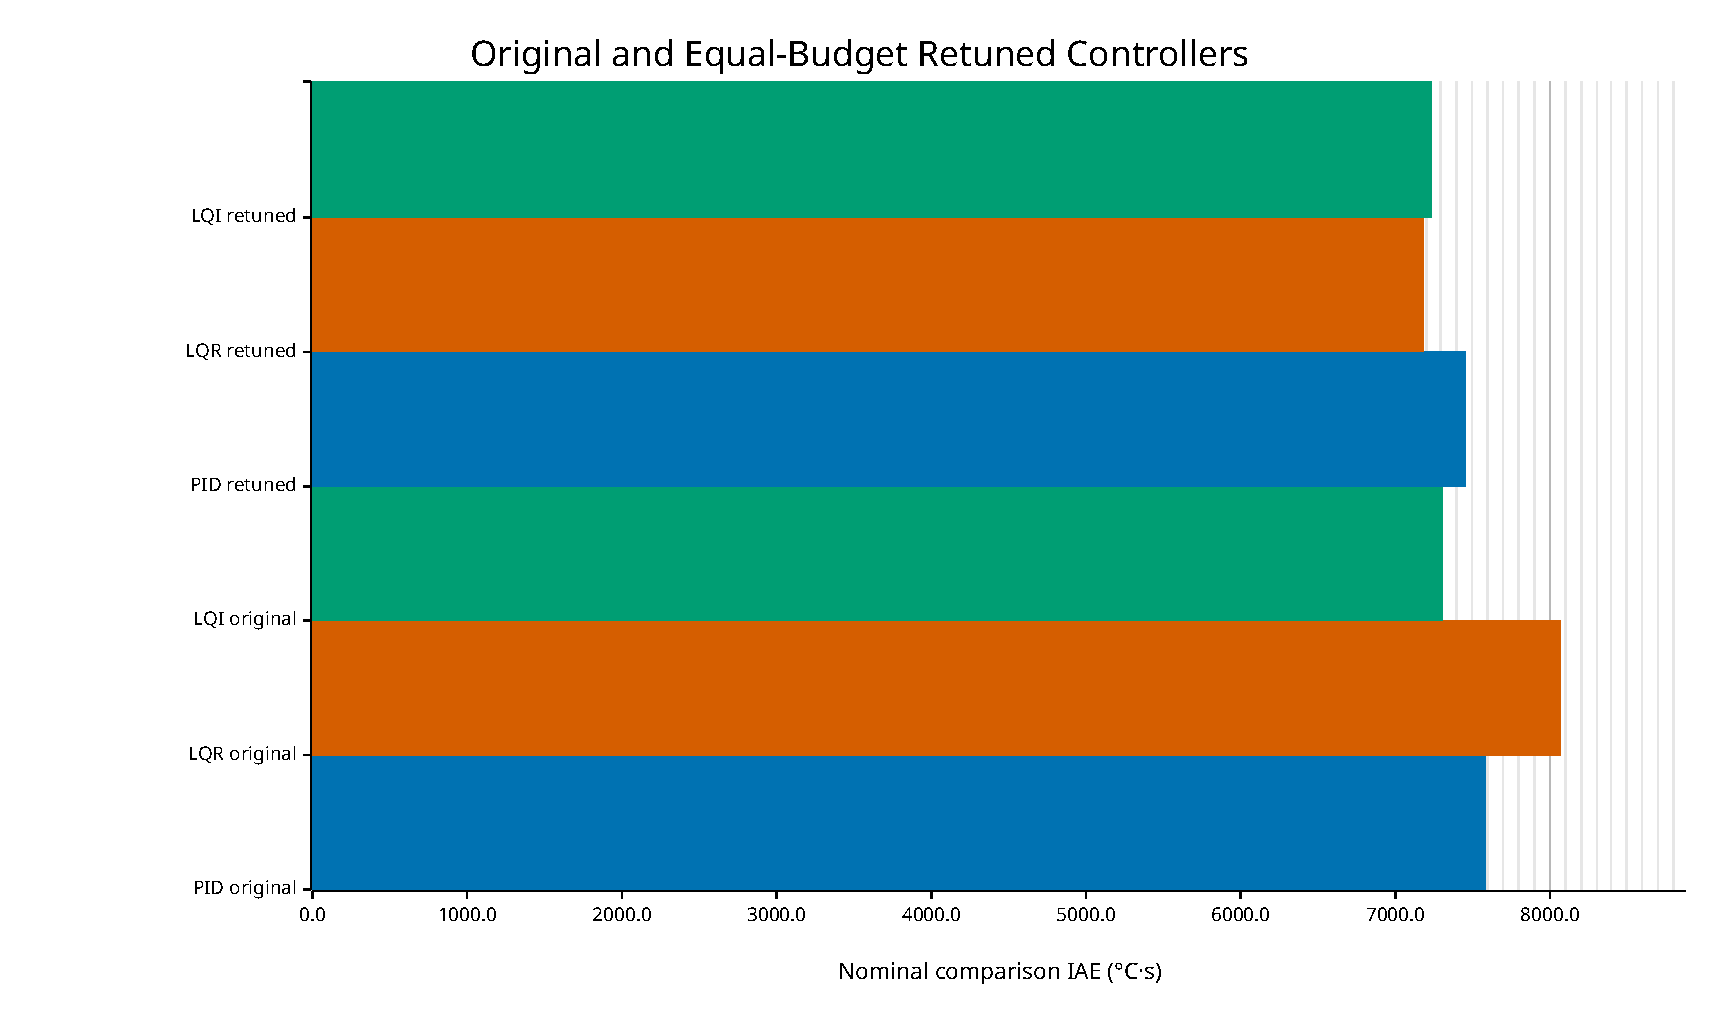
\includegraphics[width=\linewidth]{figures/original-vs-retuned.pdf}\caption{기존 및 동일 예산 재튜닝 공칭 IAE.}\label{fig:tuning}\end{figure}

\subsection{불확실성과 일정 부하 제거}
열용량 불확실성에 따른 기존 제어기의 RMSE 범위 변화는 PID, LQR, LQI 각각 1.824, 1.898, \SI{1.878}{\celsius}이고, 같은 백분율의 $UA$ 변화에서는 0.196, 0.276, \SI{0.203}{\celsius}이다. 시험 영역의 고정 시간 지표에서는 열용량의 영향이 더 크다(\cref{fig:uncertainty}).
\begin{figure*}[!t]\centering
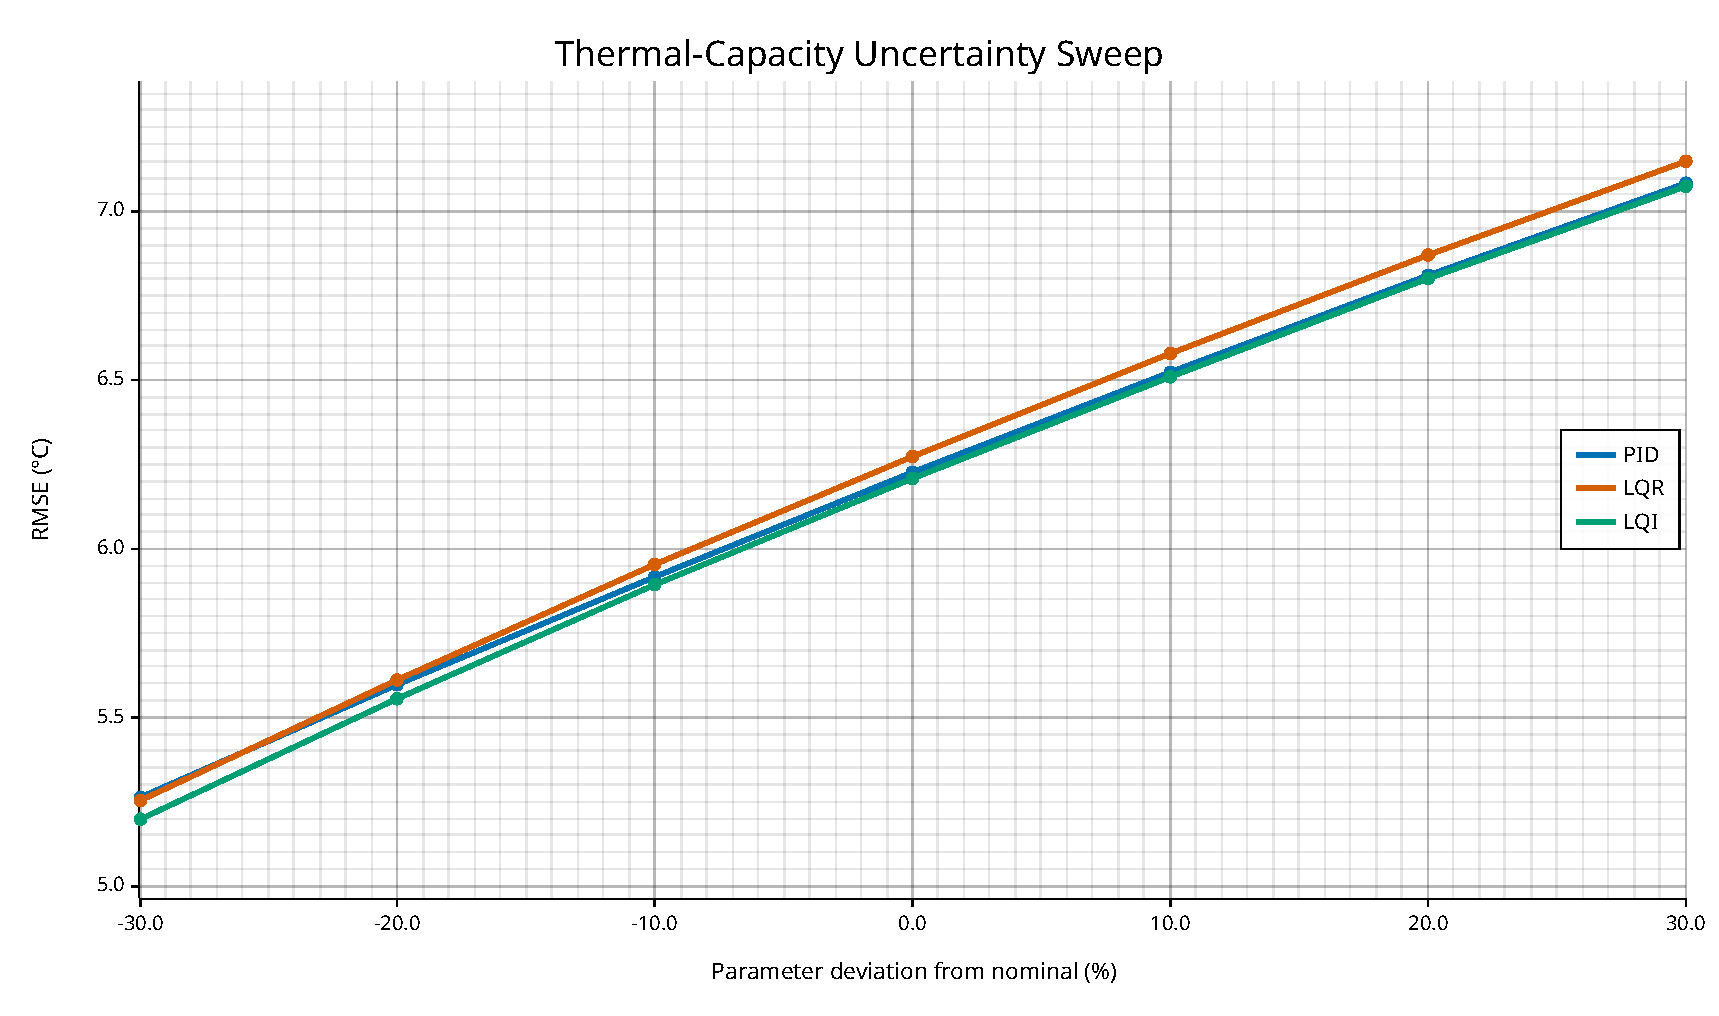
\includegraphics[width=.49\textwidth]{figures/capacity-uncertainty.pdf}\hfill
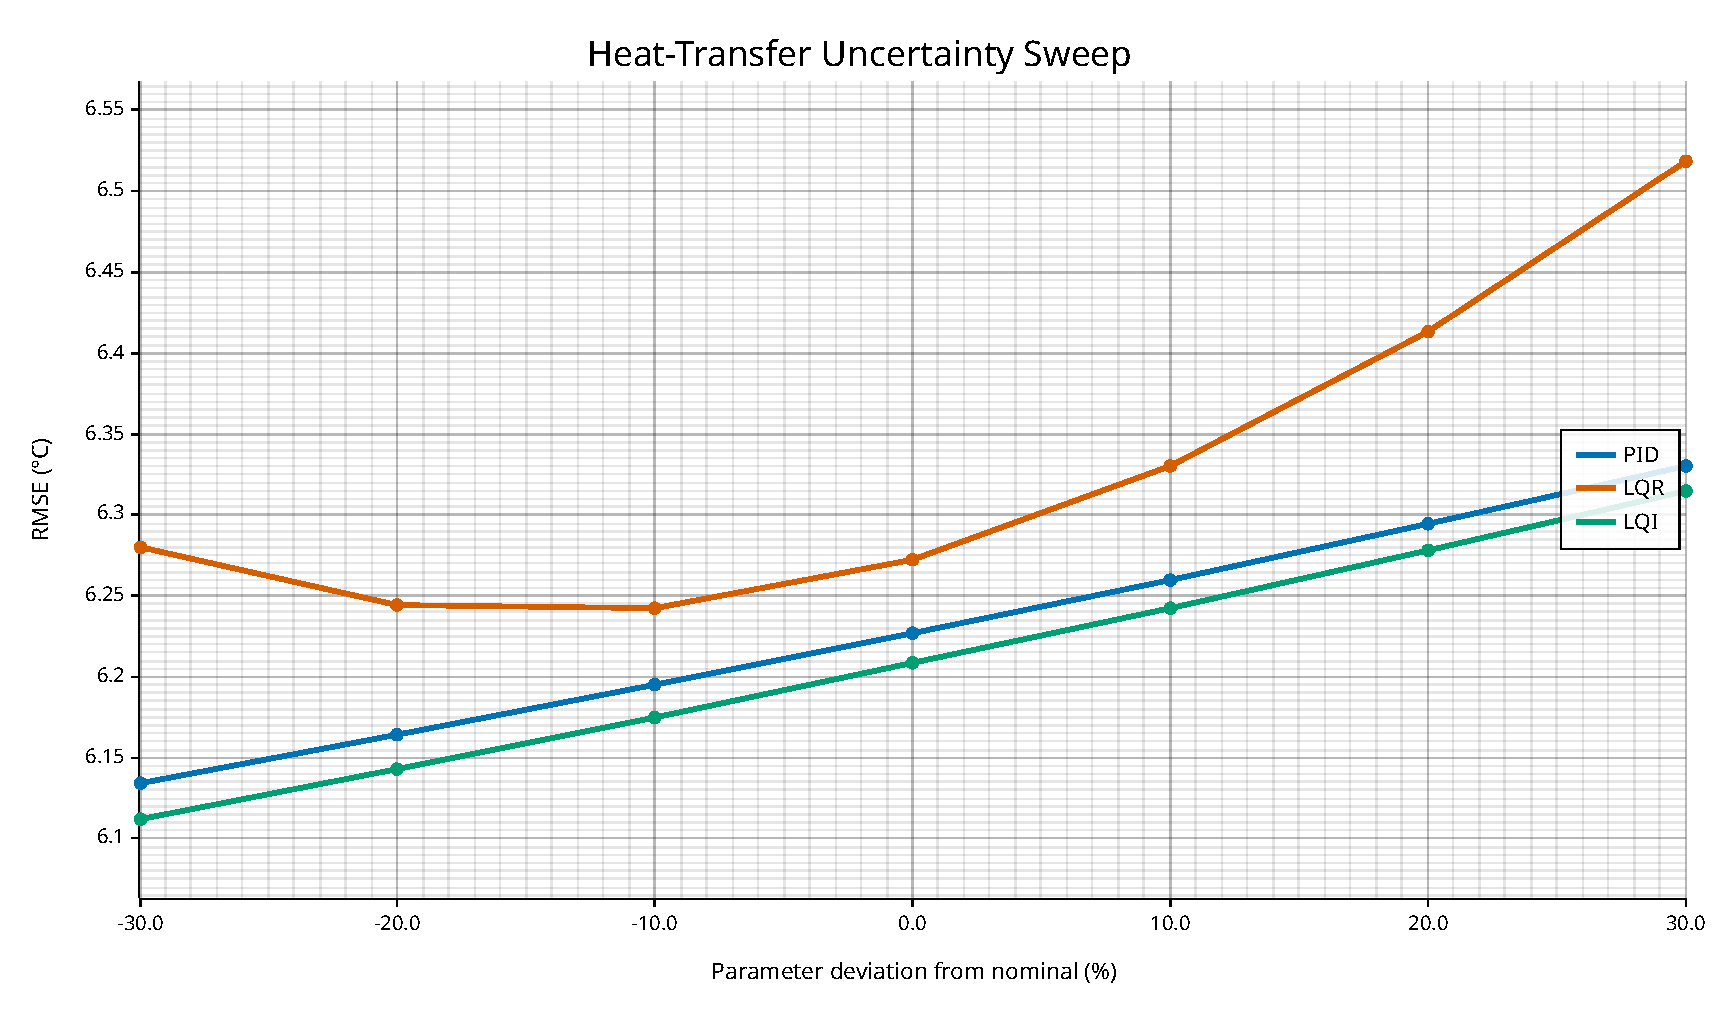
\includegraphics[width=.49\textwidth]{figures/heat-transfer-uncertainty.pdf}
\caption{열용량(왼쪽) 및 열전달(오른쪽) 불확실성에 대한 RMSE 민감도.}\label{fig:uncertainty}\end{figure*}

$-\SI{700}{W}$ 시험 부하 후 기존 제어기의 계단 이후 IAE는 PID 365.1, LQR 5006.4, LQI 118.9~$^\circ$C s이다. 말단 오차는 각각 약 0, 3.099, \SI{0}{\celsius}이다. 재튜닝 LQR은 훨씬 강한 비례 피드백으로 말단 오차를 \SI{0.079}{\celsius}까지 줄이지만 구조적 적분 제거 능력은 없다.
\begin{figure}[!htbp]\centering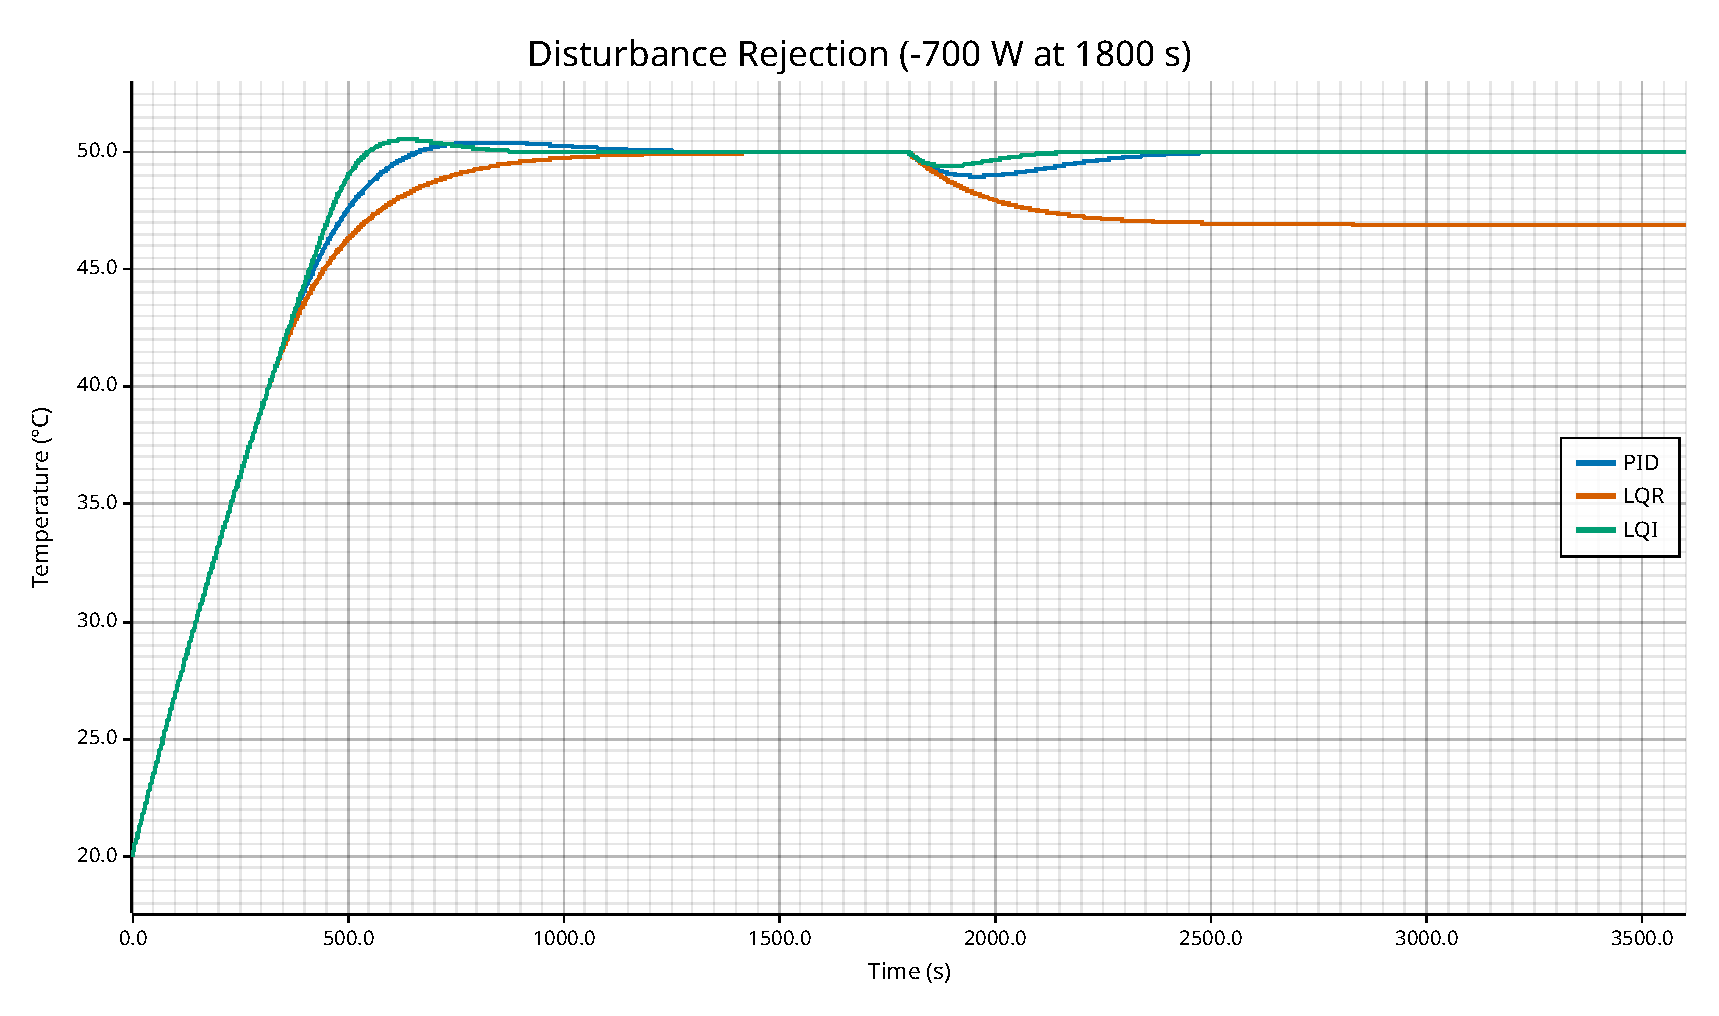
\includegraphics[width=\linewidth]{figures/disturbance-rejection.pdf}\caption{\SI{1800}{s}에서 $-\SI{700}{W}$ 부하에 대한 기존 제어기 응답.}\label{fig:disturbance}\end{figure}

\subsection{포화와 잡음}
수정된 기존 제한 액추에이터 IAE는 PID 25231.4, LQR 25268.5, LQI 25209.8~$^\circ$C s이다. 감사 전 LQR이 우세하다는 주장은 잘못된 안티와인드업 한계에서 비롯되었다. 재튜닝 제한 액추에이터 순위는 LQR(25200.3), LQI(25204.6), PID(25221.5)이며, 재튜닝 공칭 결과와 비교해 작은 순위 변화가 있다. 공통적으로 포화가 지배하는 과도응답에 비하면 차이는 매우 작다.
\begin{figure}[t]\centering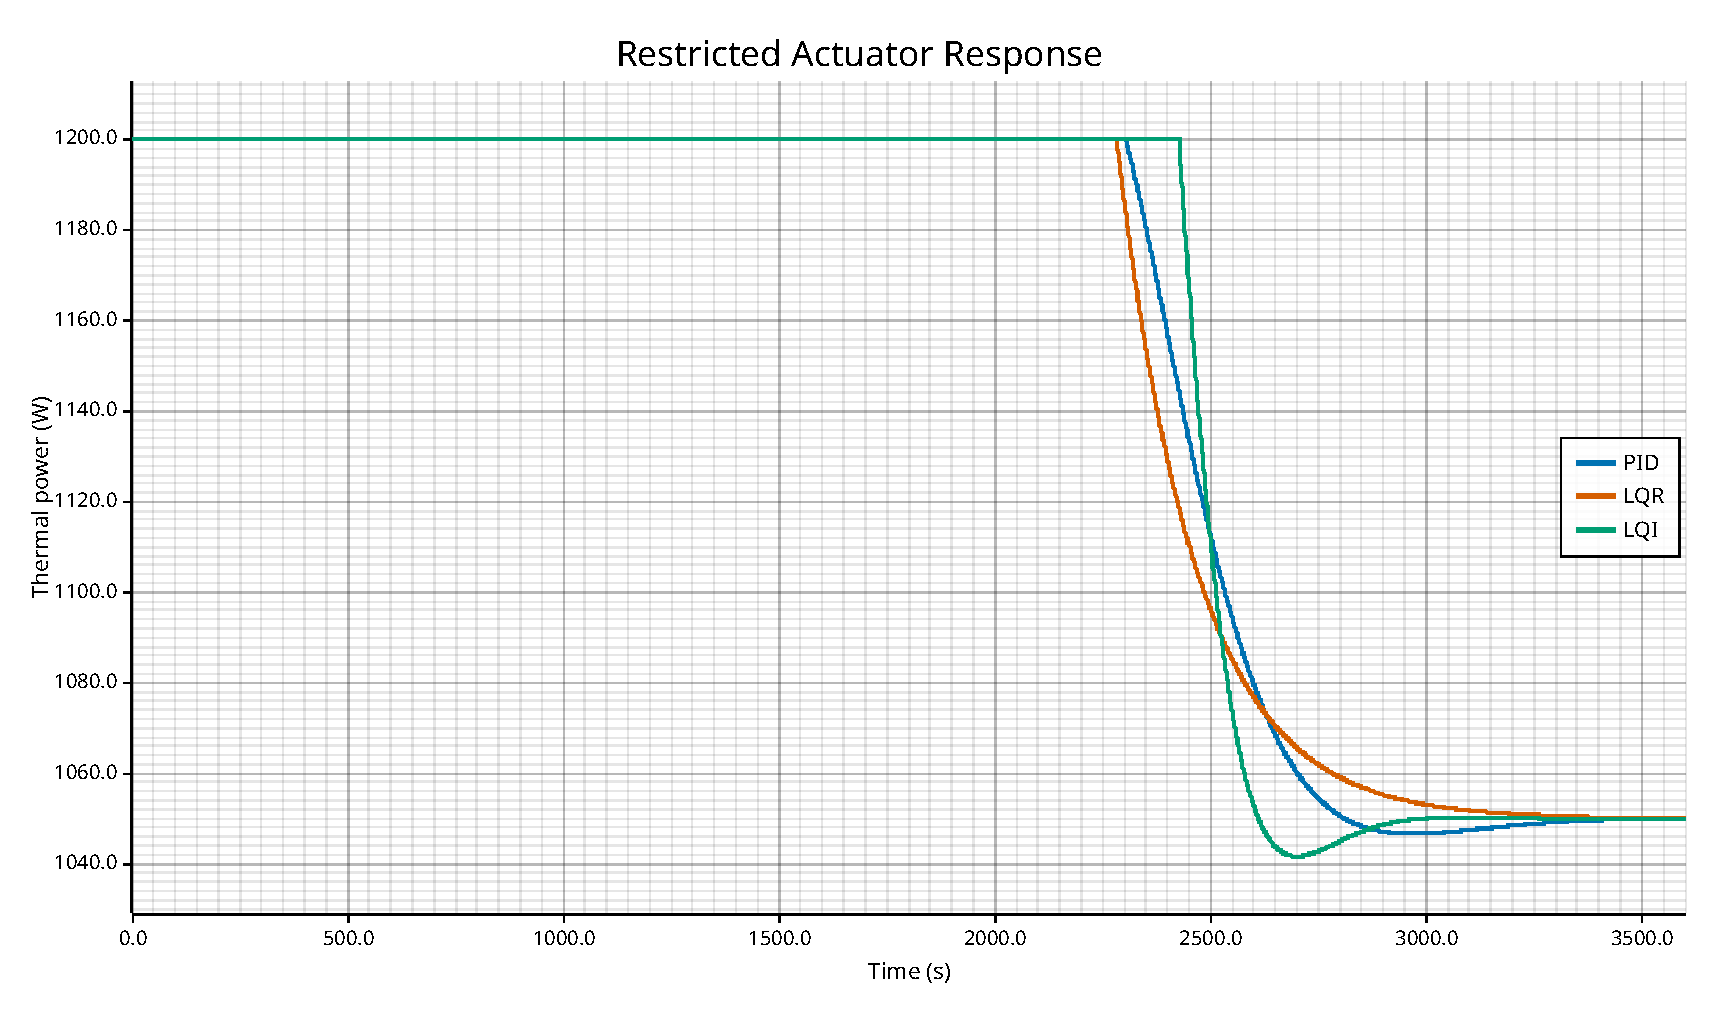
\includegraphics[width=\linewidth]{figures/actuator-saturation.pdf}\caption{제한된 한계에서 기존 제어기의 인가 동력.}\label{fig:saturation}\end{figure}

정상 구간에서 LQI와 PID의 짝지은 잡음 RMSE 차이는 \SI{0.004216}{\celsius}이다(95\% 신뢰구간 0.003978--0.004453, $d_z=3.52$). 반복 변동성이 매우 작아 표준화 효과크기는 크지만, 0.004도는 이 이상 공정에서 실용적으로 무시할 만하다. 잡음 크기나 스펙트럼이 달라지면 결론도 달라질 수 있으므로 센서 일반에 대한 주장은 하지 않는다.
\begin{figure}[t]\centering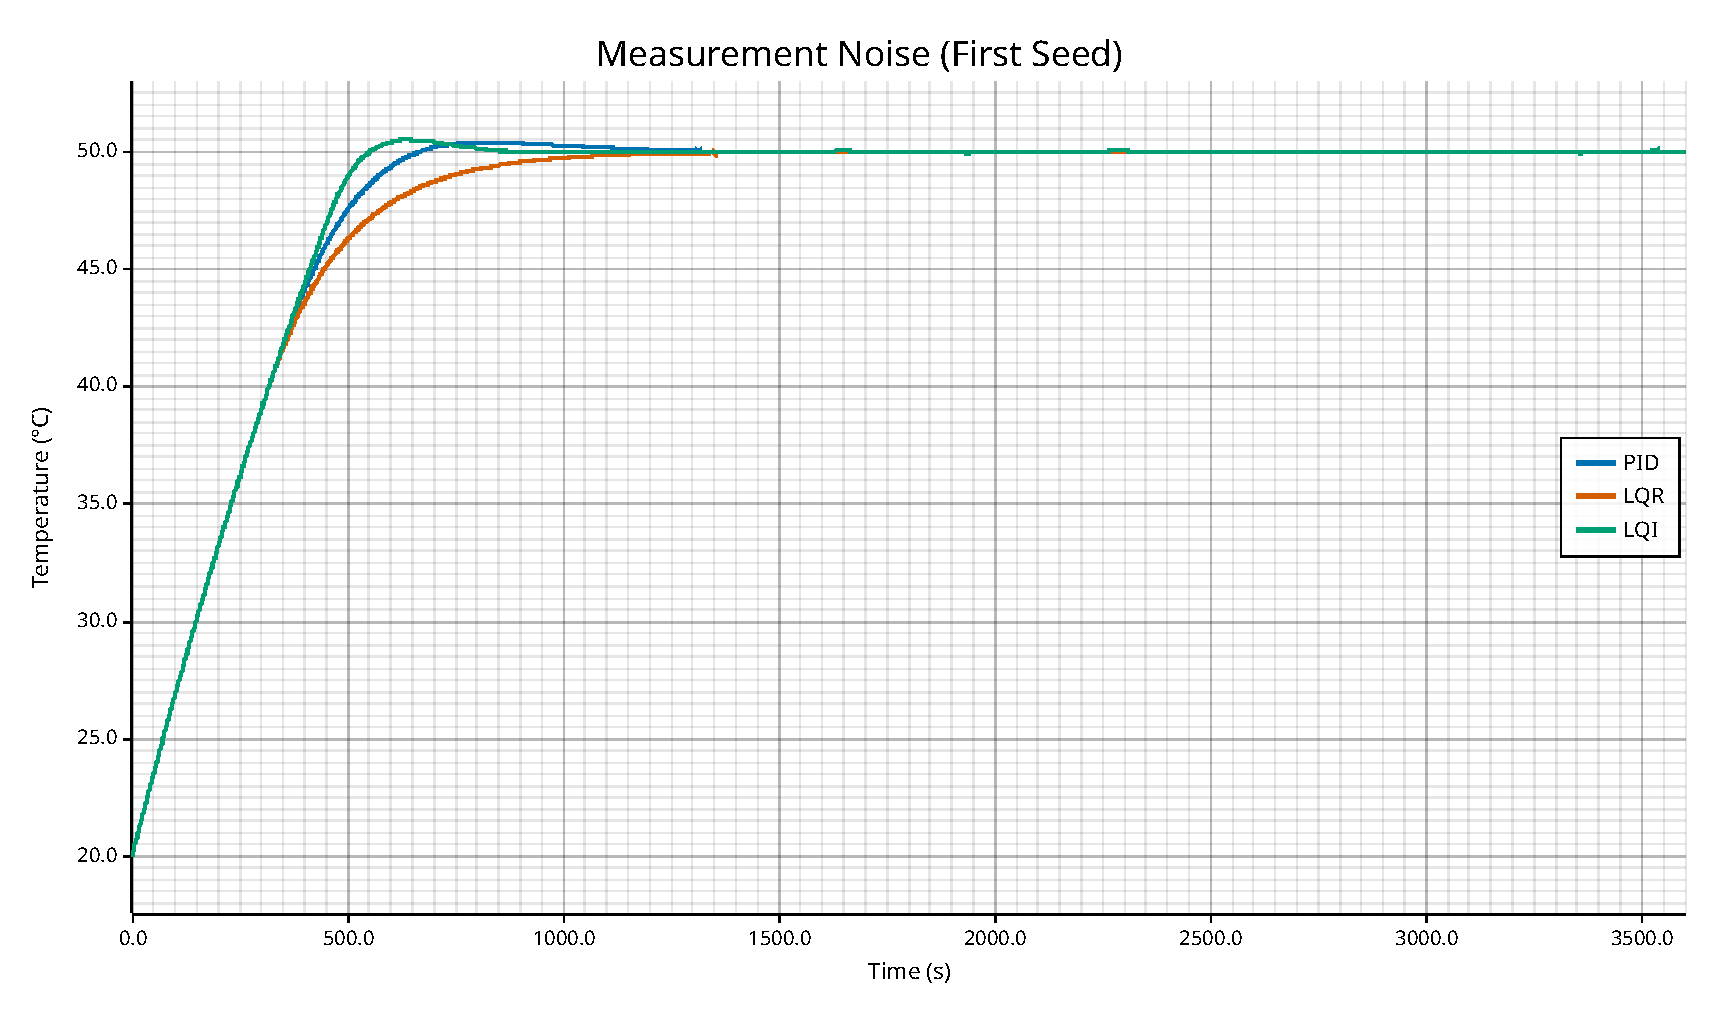
\includegraphics[width=\linewidth]{figures/measurement-noise.pdf}\caption{\SI{0.15}{\celsius} 측정 잡음의 한 짝지은 실현.}\label{fig:noise}\end{figure}

\subsection{모델에 포함되지 않은 센서 동특성}
지연 공정은 재튜닝 상충관계를 드러낸다(\cref{tab:fidelity,fig:fidelity}). 재튜닝 LQR IAE는 9345.2~$^\circ$C s로 증가하고 정착하지 않으며 2739~s 동안 포화된다. 기존 LQR IAE는 7804.1이다. PID와 LQI 변화는 훨씬 작다. 공격적인 공칭 튜닝은 단순 공정 성능을 높이지만 누락된 센싱 동특성에 대한 허용도를 낮춘다.
\begin{table}[!htbp]\centering\caption{Rust로 생성한 센서 지연 결과.}\label{tab:fidelity}\resizebox{\linewidth}{!}{\begin{tabular}{llrrr}\toprule
Design & Controller & IAE ($^\circ$C s) & RMSE ($^\circ$C) & Saturation (s) \\
\midrule
Original & PID & 7447.1 & 6.218 & 365 \\
Original & LQR & 7804.1 & 6.245 & 344 \\
Original & LQI & 7289.2 & 6.208 & 488 \\
Retuned & PID & 7364.1 & 6.215 & 395 \\
Retuned & LQR & 9345.2 & 6.252 & 2739 \\
Retuned & LQI & 7295.1 & 6.208 & 507 \\
\bottomrule\end{tabular}
}\end{table}
\begin{figure}[t]\centering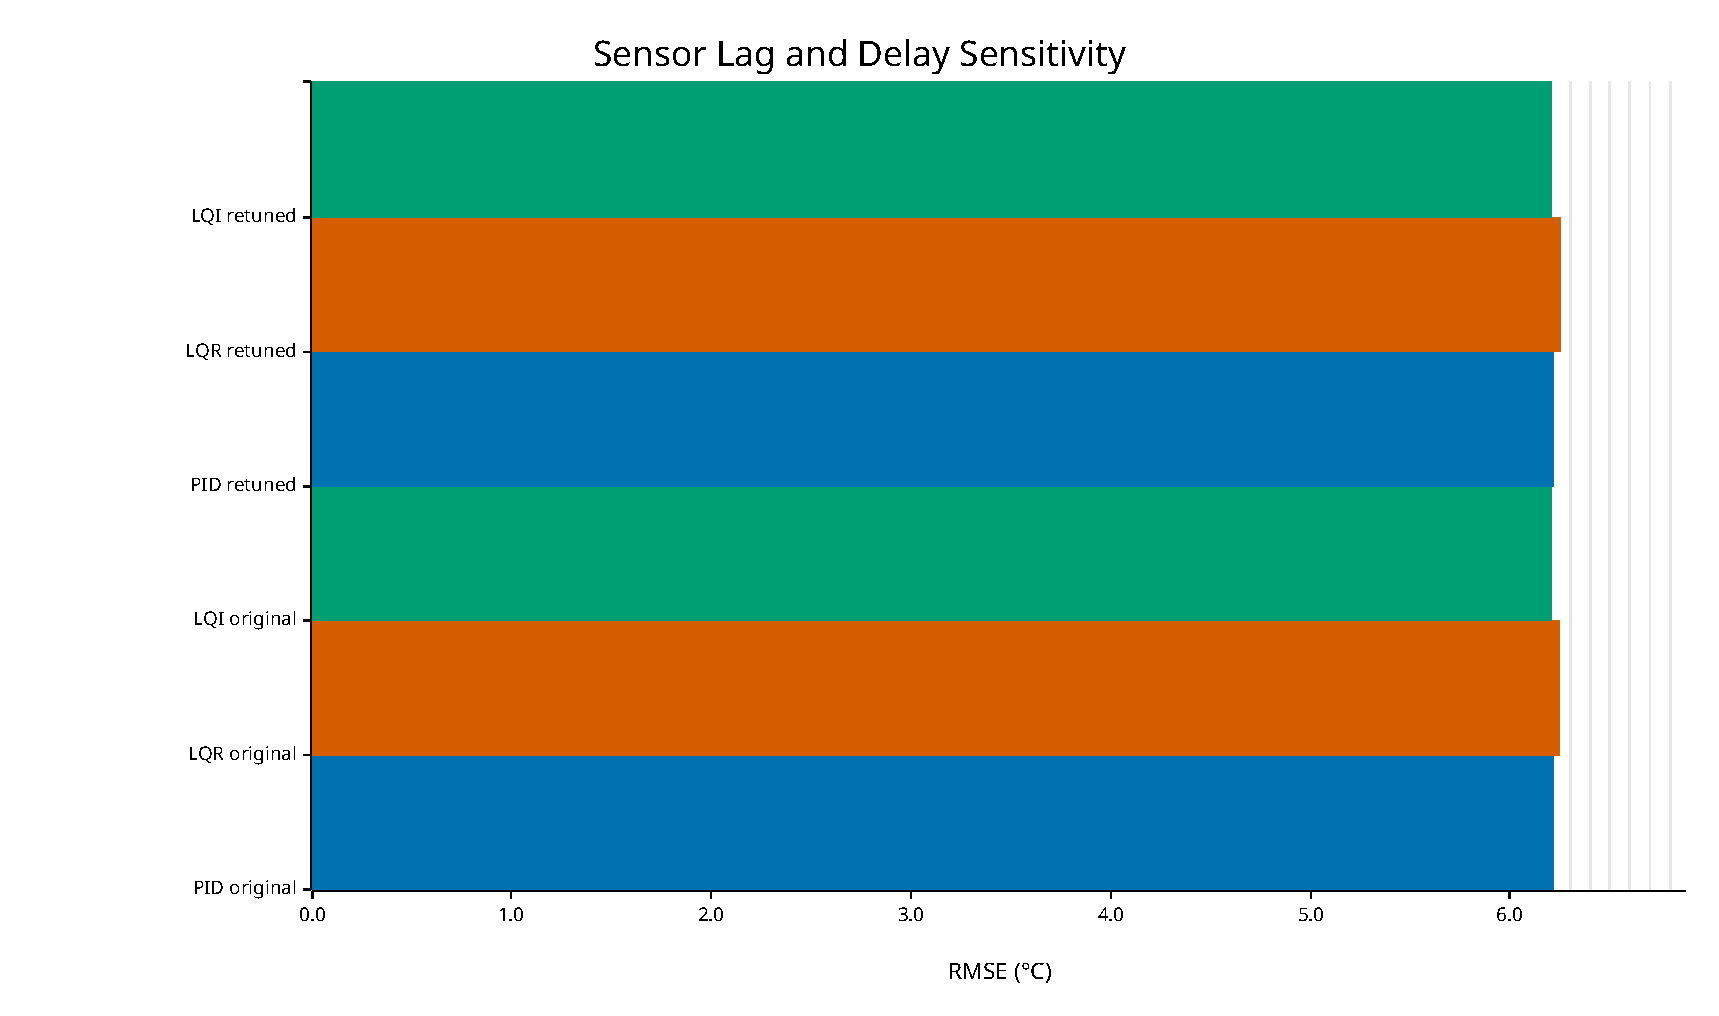
\includegraphics[width=\linewidth]{figures/higher-fidelity-summary.pdf}\caption{\SI{20}{s} 센서 지연과 \SI{10}{s} 순수 지연에서의 RMSE.}\label{fig:fidelity}\end{figure}
\FloatBarrier
